\section{Agricultural Remote Sensing}
\label{sec:ag_contextualization}

\fromsurvey{\ac{RS} can be defined as the field that studies, from a distance, objects and phenomena \citep{Jensen2014}. Remotely sensed data can be acquired from non-contact sensor systems, such as satellites, planes, and drones. All sensors are based on the study of \ac{EMR} and the ability of individual targets to reflect, absorb, and transmit this \ac{EMR} \citep{Jensen2014, Brandt2009}. According to the authors, there are two main types of sensors: (i) passive and (ii) active. Passive sensors are those that can only receive \ac{EMR}, such as optical and thermal sensors. Active sensors are those that can transmit and receive \ac{EMR}, such as \ac{SAR} and \ac{LiDAR}\footnote{Please refer to Jensen \citep{Jensen2014}.}.}

\fromdatacentricai{Except for \ac{LiDAR} data, remote sensing images are usually stored as raster files, usually in TIFF \citep{poynton1992overview} or NetCDF \citep{rew1990netcdf} formats. The term ``raster'' originally comes from the Latin rastrum, meaning ``rake,'' referring to something that ``sweeps'' a surface. In the context of computer graphics and geotechnology, it has been adopted to describe how digital images are organized in a matrix structure \citep{jensen2015introductory, novo2013sensoriamento}. The adoption of the term is also related to the process of acquiring remote sensing images, which often occurs through line-by-line scanning, similar to a systematic sweeping of the terrain.}

\fromsurvey{\ac{LiDAR} and \ac{SAR} sensors are known to be very useful for remotely sensed data. The former is filling an enormous gap in remotely sensed data: more accurate height variations, i.e. 3D data \citep{wangChallengesOpportunitiesLidar2021}. These 3D data can be used to estimate crops and canopy height, which, in its turn, is used for biomass estimation \citep{riveraLiDARApplicationsPrecision2023}. As for the latter, \ac{SAR}, \cite{liuResearchAdvancesSAR2019} explain that \ac{SAR} \ac{EMR} can penetrate clouds, which enables crop monitoring throughout the year without interference. The authors also stated that \ac{SAR} has been quite useful for crop identification because its backscatter is affected by biomass structure, solid condition and provides improved accuracy when used with different polarizations.}

\fromsurvey{Even though \ac{SAR} and \ac{LiDAR} sensors are extremely useful for remote sensing, they are not yet widely used due to their revisit time, which is lower than optical satellite data \citep{Jensen2014}}, This limitation has been further exacerbated by the reported malfunction of one of the most widely used \ac{SAR} sensors, Sentinel-1B, which became inoperative on December 23, 2021 \footnote{Mission ends for Copernicus Sentinel-1B satellite - \url{https://www.esa.int/Applications/Observing_the_Earth/Copernicus/Sentinel-1/Mission_ends_for_Copernicus_Sentinel-1B_satellite}}, resulting in a significant data gap, particularly in some regions (see Table \ref{tab:context-satellites}). \fromsurvey{Another drawback is that their process is far more complex than optical data. \ac{SAR} data needs to be chosen according to the necessity: the polarization, ascending or descending orbit, single look complex, etc. This data is also provided in \ac{dB}, a logarithmic scale. Besides, \ac{SAR} usually follows the Rayleigh distribution \citep{kuruogluModelingSARImages2004}, unlike most optical data that follow the normal distribution. This indicates preprocessing for \ac{SAR} data, which requires computational effort and specific knowledge for processing it. As for \ac{LiDAR} data, it is a point cloud that needs to be processed into a model to be later used as an input for machine learning models  \citep{riveraLiDARApplicationsPrecision2023}. In a nutshell, both \ac{SAR} and \ac{LiDAR} data are not as easy to process and explain as optical data is.}

\fromsurvey{When it comes to optical sensors, we can study how each target can respond to each size of electromagnetic wave, which usually vary from \ac{VIS} - from 450 to 750 nm - to \ac{NIR} - from 750 to 1300 nm - by its reflectance value. Based on that, researchers could describe the spectral behavior for each target, in a sense that the analyst can distinguish types of land cover (eg. water, vegetation, bare soil) and understand its characteristics \citep{plants12122347}. From these different spectral responses, it is even possible to differentiate crops, as shown in Figure \ref{fig:context_reflectances1}. This Figure presents different patterns for each type of crop (corn, sugarcane, coffee, canola, wheat, tobacco) according to their respective factor of reflectance.}

\fromsurvey{For a thorough observation in Figure \ref{fig:context_reflectances1}, wheat is more easily distinguished from the other crops, once its reflectance is higher for almost all wavelengths, mainly \ac{NIR} and \ac{SWIR}. On the other hand, tobacco can be distinguished better at \ac{VIS}, in wavelengths close to yellow and so forth.}

\begin{figure}[!ht]
    \centering
    \caption{\fromsurvey{Example of spectral behavior of different crops classes.}}
    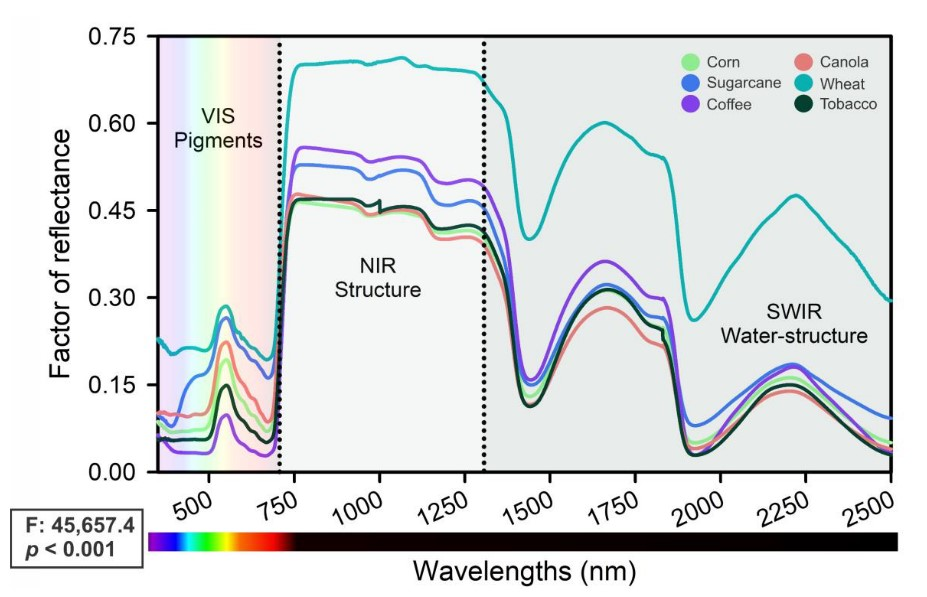
\includegraphics[width=0.95\linewidth]{figures/3_theoretical_background/veg_reflectance.jpg}
    \fignote{ The wavelengths refer to: visible (VIS), near-infrared (NIR) and short-wave infrared (SWIR). Adapted from \cite{plants12122347}}
    \label{fig:context_reflectances1}
\end{figure}

\subsection{Vegetation Indices}

\fromsurvey{From the spectral reflectance, researchers studied methods for better understanding targets and how to discriminate them. They created vegetation indices that, for agriculture, can help analysts to describe vegetation health and age. These indices aim to highlight part of the image with different vegetation cover; they are usually obtained by dividing two spectral bands with high and low reflectance values, respectively \citep{bannari1995review,gao2020remote, ReflectanciaDosMateriais2021}. They are related to spectral estimates for biochemical and biophysical analyses, such as the chlorophyll content and biomass \citep{ndvi1}. Wavelengths approximately between 700 nm up to 1400 nm (\ac{NIR} and \ac{SWIR}) reflect better vegetation than other land covers, such as dry soil and water, while red wavelengths ($\approx$ 660 nm) do not \citep{Jensen2014}.}

\fromsurvey{Some of the most used indices are \ac{NDVI} \citep{ndvi1}, \ac{EVI} \citep{evi1}, \ac{EVI2} \citep{evi2} and \ac{NDYI} \citep{ndyi1} As previously mentioned, all of them consider bands with high reflectance and low reflectance, respectively. \ac{NDVI} was one of the first indices used in \ac{RS}, using red reflectance values ($\rho_{red}$) and \ac{NIR} ($\rho_{NIR}$); it is presented in Equation \ref{eq:ndvi}. This index is extensively used for agriculture, and it has proven to indicate start of seasons and concern for field assessments \citep{FAOfoodandagricultureorganizationoftheunitednationsGuidelinesUseRemote2018}. On the other hand, \ac{EVI} uses the blue reflectance  ($\rho_{blue}$) together with aerosol resistance ($C_1$ and $C_2$) and canopy background ($L$); it is adjusted not to saturate in high-density canopy cover (Equation \ref{eq:evi}). \ac{EVI2} adjusted \ac{EVI} to only two bands, and the authors state that there is no statistical difference between them. As can be seen, if $L=0$, then \ac{EVI2} is very similar to \ac{NDVI}. \ac{EVI} and \ac{EVI2} are used. In general, \ac{NDVI} usually highlights crop flourishing and indicates the amount of humidity in the parcel. On the other hand, \ac{NDYI}, \ac{EVI} and \ac{EVI2} are used to highlight and understand vegetation peaks of crops and differentiate dense structures.}


\begin{equation}
\label{eq:ndvi}
    NDVI = \frac{\rho_{NIR} - \rho_{red}}{\rho_{NIR} + \rho_{red}}
\end{equation}

\begin{equation}
\label{eq:evi}
        EVI = 2.5 \frac{\rho_{NIR} - \rho_{red}} {L + \rho_{NIR} + C_1\rho_{red}-C_2\rho_{blue}}
\end{equation}

\begin{equation}
\label{eq:evi2}
    EVI2 = 2.5 \frac{\rho_{NIR} - \rho_{red}}{\rho_{NIR} + \rho_{red} + L}
\end{equation}

\begin{equation}
\label{eq:ndyi}
    NDYI = \frac{\rho_{green} - \rho_{blue}}{\rho_{green} + \rho_{blue}}
\end{equation}

\subsection{Earth Observation Satellites}
\label{sec:context_satellites}

\fromsurvey{Since the 1970s, earth observation satellites have been developed to monitor target tasks with specific spectral responses, including vegetation, soil, water, and climate variables. The United States' \ac{NASA} initiated the Landsat program in 1972, creating the longest continuous global land observation record \citep{masek2020,wulder2022}, while its \ac{EOS} expanded capabilities with sensors like \ac{MODIS} and \ac{ASTER} \citep{nasa2020}. The \ac{ESA} developed the Copernicus program with its Sentinel satellite series (2014-present) for open global monitoring \citep{esa2021}, building on earlier ERS and Envisat missions \citep{attema2007}. China's CNSA (China National Space Administration) deployed the Gaofen series (2013-present) and collaborated with Brazil's \ac{INPE} on the \ac{CBERS} program (since 1999) \citep{li2022,lino2000cbers}, with Brazil later launching its first independent satellite Amazonia-1 in 2021 \citep{amazonia2021}. France's \ac{CNES} pioneered commercial high-resolution imaging through \ac{SPOT} (1986-2012) and Pleiades (2011-present) satellites \citep{spot2012,gleyzes2012pleiades}, while India's \ac{ISRO} established regional monitoring via its \ac{IRS} program (1988-present) \citep{navalgund2007}. Also, \ac{JAXA} has missions such as the \ac{ALOS}, a program started in 2006, aiming to provide data for environmental and resource sciences.}


\fromsurvey{
Most EO optical satellites feature specific spectral bands, called \textbf{spectral resolution} \citep{jensen2016}, for different wavelengths:
\begin{itemize}
    \item \textbf{Blue} ($\approx 450-520$ nm),
    \item \textbf{Green} ($\approx 520-600$ nm),
    \item \textbf{Red} ($\approx 630-690$ nm),
    \item \textbf{Near-infrared} (NIR, $\approx 760-1300$ nm),
    \item \textbf{Shortwave infrared} (SWIR, $\approx 1550-1750$ nm and $\approx 2080-2350$ nm).
\end{itemize}}

\fromsurvey{Another crucial aspect of all kinds of remote sensing data is the \textbf{spatial resolution} (the length of one pixel side), classified as:
\begin{itemize}
    \item \textbf{\Acf{VHR}}: $\leq$ 2 m (e.g., WorldView-4),
    \item \textbf{\Acf{HR}}: 2-10 m (e.g., Sentinel-2),
        \item \textbf{\Acf{MR}}: 10-100 m (e.g., Landsat-9),
        \item \textbf{\Acf{LR}}: $\geq$ 100 m (e.g., MODIS) \citep{belward2015}.
\end{itemize}}

\fromsurvey{Also, a critical parameter is the imaging frequency for a given area \citep{wulder2019}, called \textbf{temporal resolution} or \textbf{revisit time}.}

\fromsurvey{The Earth observation data ecosystem includes significant contributions from private companies such as Planet, Maxar, and Airbus, which operate constellations from low up to high-resolution satellites \citep{planet2023,maxar2022,airbus2021}. While these commercial systems provide valuable capabilities for specific applications, our study focuses exclusively on publicly available datasets from programs like Landsat  - \ac{NASA}/\ac{USGS} -  and Sentinel (\ac{ESA}), which offer long-term, research-friendly, open data policies essential for scientific research and global environmental monitoring \citep{masek2020,esa2021}. This emphasis on open data ensures reproducibility and equitable access to Earth observation information across the scientific community. In this direction, some recent initiatives like the \ac{BDC} and \ac{AGDC} simplified \ac{EO} data access by providing easy-to-consume, analysis-ready multitemporal and multisensor data cubes \citep{camara2020,giuliani2020earth}.}

\fromsurvey{Table \ref{tab:context-satellites} summarizes the main satellites referenced in this review, with consolidated information from the \textbf{eoPortal}\footnote{\url{https://www.eoportal.org/}} catalog \citep{eoportal2023}.}


\begin{table}[!ht]
\centering
\caption{\fromsurvey{Main satellite missions used by the selected datasets.}}
\label{tab:context-satellites}

\resizebox{\textwidth}{!}{
\begin{tabular}{lllllllllll}
\hline
\textbf{Mission} && \textbf{Launch} && \textbf{Sensor}&& \textbf{\begin{tabular}[c]{@{}l@{}}Spatial\\ Resolution\end{tabular}} && \textbf{\begin{tabular}[c]{@{}l@{}}Spectral\\ Resolution\end{tabular}}&& \textbf{\begin{tabular}[c]{@{}l@{}}Revisit\\ (days)\end{tabular}} \\ \hline
Landsat-1 (L1)*&& 1972&& MSS&& $\sim$80 m&& VIS, NIR&& 18\\ \hline
Landsat-2 (L2)*&& 1975&& MSS&& $\sim$80 m&& VIS, NIR&& 18\\ \hline
Landsat-3 (L3)*&& 1978&& RBV&& \begin{tabular}[c]{@{}l@{}}$\sim$40 m,\\ $\sim$80 m\end{tabular}&& PAN, VIS, NIR && 18\\ \hline
Landsat-4 (L4)*&& 1982&& TM && $\sim$30 m&& \begin{tabular}[c]{@{}l@{}}VIS, NIR,\\ SWIR, Thermal\end{tabular} && 16\\ \hline
Landsat-5 (L5)*&& 1984&& TM && $\sim$30 m&& \begin{tabular}[c]{@{}l@{}}VIS, NIR,\\ SWIR, Thermal\end{tabular} && 16\\ \hline
SPOT && 1986&& \begin{tabular}[c]{@{}l@{}}HRV, HRVIR,\\ Vegetation\end{tabular} && 1.5-20 m&& VIS, NIR&& 2-3 \\ \hline
POES, MetOp&& 1998&& AVHRR&& $\sim$1.1 km&& VIS, NIR, Thermal && 0.5 \\ \hline
Landsat-7 (L7) && 1999&& ETM+ && $\sim$30 m&& \begin{tabular}[c]{@{}l@{}}VIS, NIR,\\ SWIR, Thermal\end{tabular} && 16\\ \hline
MODIS&& 1999&& Terra, Aqua&& \begin{tabular}[c]{@{}l@{}}250 m, 500 m\\ 1 km\end{tabular} && \begin{tabular}[c]{@{}l@{}}VIS, NIR,\\ SWIR, Thermal\end{tabular} && 1-2 \\ \hline
QuickBird-2&& 2001&& Pan, Ms&& \begin{tabular}[c]{@{}l@{}}0.61 m,\\ 2.44 m\end{tabular}&& VIS, NIR&& 3-7 \\ \hline
ALOS && 2006 &&  \begin{tabular}[c]{@{}l@{}}PALSAR (L-band)\\ AVNIR-2 \\ PRISM\end{tabular} && \begin{tabular}[c]{@{}l@{}}7-44 m\\ 10 m \\ 2.5 m\end{tabular} &&  \begin{tabular}[c]{@{}l@{}}HH+HV or VV+VH\\ RGB-NIR \\ PAN\end{tabular} && 46\\ \hline 
GeoEye-1 && 2008&& MS, PAN&& \begin{tabular}[c]{@{}l@{}}0.41 m,\\ 1.65 m\end{tabular}&& VIS, NIR&& 3-5 \\ \hline
WorldView-2(WV2) && 2009&& Pan, Ms&& \begin{tabular}[c]{@{}l@{}}0.46 m,\\ 1.84 m\end{tabular}&& VIS, NIR&& 1.1 \\ \hline
\begin{tabular}[c]{@{}l@{}}Suomi-NPP,\\ NOAA-20\end{tabular} && 2011&& VIIRS&& 375 m && \begin{tabular}[c]{@{}l@{}}VIS, NIR,\\ SWIR, Thermal\end{tabular} && 1 \\ \hline
Landsat-8 (L8) && 2013&& OLI, TIRS&& $\sim$30 m&& \begin{tabular}[c]{@{}l@{}}VIS, NIR, SWIR,\\ Thermal, Cirrus\end{tabular} && 16\\ \hline
Planet && 2013&& PlanetScope&& 3-5 m && VIS, NIR&& 1 \\ \hline
Sentinel-1 (S1)&& 2014&& SAR C-Band && 10 m&& VV, VH, HV&& 12\\ \hline
CBERS-4&& 2014&& \begin{tabular}[c]{@{}l@{}}PAN, MUX,\\ WFI\end{tabular}&& 5-20 m&& VIS, NIR&& 26\\ \hline
GaoFen-2 (GF2)** && 2014&& PAN, MS&& \begin{tabular}[c]{@{}l@{}}1 m,\\ 4 m\end{tabular}&& VIS, NIR&& 5 \\ \hline
WorldView-3 (WV3)&& 2014&& \begin{tabular}[c]{@{}l@{}}Pan, MS,\\ SWIR\end{tabular}&& \begin{tabular}[c]{@{}l@{}}0.31 m,\\ 1.24 m,3.7 m\end{tabular}&& VIS, NIR, SWIR&& 1 \\ \hline
ALOS-2 && 2014 && PALSAR-2 (L-Band) && 10 m && HH+HV or VV+VH && 16\\ \hline
Sentinel-2 (S2)&& 2015&& MSI&& 10-60 m && \begin{tabular}[c]{@{}l@{}}VIS, NIR,\\ SWIR, RedEdge\end{tabular} && 5 \\ \hline
Sentinel-3 (S3)&& 2016&& \begin{tabular}[c]{@{}l@{}}SLSTR,\\ OLCI, SRAL\end{tabular}&& \begin{tabular}[c]{@{}l@{}}300 m,\\ 1 km\end{tabular} && \begin{tabular}[c]{@{}l@{}}VIS, NIR,\\ SWIR, Thermal\end{tabular} && 1-2 \\ \hline
CBERS-4A && 2019&& PAN, MUX && 5-10 m&& PAN, VIS, NIR && 31\\ \hline
Landsat-9 (L9) && 2021&& \begin{tabular}[c]{@{}l@{}}OLI-2,\\ TIRS-2\end{tabular}&& $\sim$30 m&& \begin{tabular}[c]{@{}l@{}}VIS, NIR, SWIR,\\ Thermal, Cirrus\end{tabular} && 16\\ \hline
ALOS-4 && 2024 && PALSAR-3 (L-Band) && 10 m && HH, HV, VV, VH && 14\\ \hline 
\end{tabular}
}
\caption*{\fromsurvey{*Out of order; **Not open access. \\ VIS: Visible; NIR: near-infrared; SWIR: short-wave infrared; PAN: panchromatic; VV, VH, HV are SAR polarizations referring to Vertical-Vertical, Vertical-Horizontal, Horizontal-Vertical, and Horizontal-Horizontal}.}
\end{table}

\subsection{Pre-existing datasets}

\fromsurvey{Datasets play a crucial role in creating a Machine Learning model, mainly for agriculture, once it can contain \textit{in-situ} data or previous knowledge of the region of interest to be created. Both cases are used for field validation; to be more specific, the \textit{in situ} data can retrieve the reflectance information of the target, creating its chart for spectral behavior \citep{Brandt2009} while field knowledge can aid in \ac{LULC} classification. During the dataset search, we did not find any other review article that mapped datasets before from the previous version of this work \citep{mateuzin2024}. Another point is that datasets tend not to generalize well from one region to another, which is related to differences in biomes, topography, climate and agricultural calendars \citep{gadiraju2023remote, kerner2024multi, huber2024leveraging}, although Transfer Learning can be beneficial \citep{gadiraju2023remote, huber2024leveraging, kerner2024multi, khaki2021simultaneous}. For this reason, we point out the importance of mapping as many datasets as possible.}

\fromsurvey{We have searched for all publicly available datasets to date, though in this study we present those considered to be the most important by either number of citations or data size. We divided those datasets into two categories: (i) labeled, created for supervised learning and (ii) non-labeled, used for representation learning, such as Self-Supervised Learning, as well as for generating synthetic data or for unsupervised learning; this second category of datasets has information of general remotely sensed data since we found a lack of agricultural specific unlabeled datasets. Table \ref{tab:context_labeled_datasets} presents a summary of labeled datasets related to agriculture, considering their respective names, applications, and regions of interest, as well as which EO satellites were used. For more information on these datasets (i.e. labeled classes, state-of-the-art methods, evaluation criteria, etc), the readers are referred to the original papers and/or landing pages for each dataset.}

\subsubsection{Labeled Datasets}\label{sec:labeled_datasets}

\fromsurvey{The filters used for selecting the labeled datasets were: (i) we kept all datasets we found of emerging countries; (ii) small datasets or with regions already in other selected datasets were not considered; (iii) datasets merged into other datasets were not considered as well, and, finally, (iv) we considered only the most recent version for each dataset. In addition to that, Table \ref{tab:context_labeled_datasets} mention models based on remotely sensed data, such as ERA5 \citep{ERA5} and ETH-GCHM \citep{mwildRegionalClimateSimulation1996}, which are climate and weather analyzes, as well as Aster \citep{asterdem} and SRTM \citep{srtm} which are elevation models based on satellite radar data. For unlabeled datasets, there were no filters for selecting them, due to their low quantity.}


\begin{table}[!ht] % [!hb]
\centering
\caption{\fromsurvey{Synthesis of Remote Sensing Labeled Datasets.}}
\label{tab:context_labeled_datasets}
\resizebox{\textwidth}{!}{
\begin{tabular}{lllllllllll}
\hline
\textbf{Name} & \textbf{Application}& \textbf{Region} & \textbf{Input data}\\ \hline
3DFGCC* \citep{ji2020learning} & Crop Mapping& China & GF2\\ \hline
AgriSen-COG \citep{selea2023agrisen} & \begin{tabular}[c]{@{}l@{}}Crop mapping,\\ Parcel Delineation\end{tabular}& \begin{tabular}[c]{@{}l@{}}Austria, Belgium, \\ Catalonia, Denmark, \\ Netherlands\end{tabular} & S2 \\ \hline
AI4Boundaries \citep{d2023ai4boundaries} & Parcel Delineation& \begin{tabular}[c]{@{}l@{}}Western Europe, \\ Scandinavia\end{tabular}& S2, Aerial \\ \hline
BreizhCrops \citep{breizhcrops2020}& \begin{tabular}[c]{@{}l@{}}Crop Mapping,\\ Parcel Delineation\end{tabular}& Brittany& S2 \\ \hline
Crop Yield Prediction USA \citep{selea2023agrisen} & Crop Yielding & USA & Pixel level\\ \hline
Cropharvest \citep{tseng2021cropharvest} & Crop Mapping& Worldwide & S1, S2, ERA5, SRTM Elevation \\ \hline
CropNet \citep{fudong:kdd24:crop_net}& Crop Yielding & USA & S2, weather, yielding\\ \hline
DENETHOR \citep{kondmann2021denethor}& \begin{tabular}[c]{@{}l@{}}Crop Mapping,\\ Parcel Delineation\end{tabular}& Germany & S1, S2, Planet \\ \hline
Fields of The World (FTW) \citep{kerner2024fields} & \begin{tabular}[c]{@{}l@{}}Parcel Delineation,\\ Crop Mapping\end{tabular}& Worldwide & S2 \\ \hline
Global dataset of historical yields \citep{iizumi2020global} & Crop Yielding & Worldwide & County \\ \hline
LEM+ \citep{oldoni2020lem+}& Crop Mapping& Brazil& Plot level \\ \hline
PASTIS-HD \citep{garnot2021panoptic} & \begin{tabular}[c]{@{}l@{}}Crop Mapping,\\ Parcel Delineation\end{tabular}& French& S1, S2, SPOT VHR \\ \hline
Purdue Agro-climatic (PAC) \citep{LIU201761} & Crop Yielding & USA Corn Belt & \begin{tabular}[c]{@{}l@{}}Weather, Soil moisture,\\ soil temperature\end{tabular} \\ \hline
S4A \citep{sykas2022sentinel}& \begin{tabular}[c]{@{}l@{}}Crop Mapping, \\ Parcel Delineation\end{tabular} & Catalonia, France & S2 \\ \hline
Sentinel 2 Crop Mapping \citep{gallo2022in_season} & Crop Mapping& Lombardia & S2 \\ \hline
SICKLE \citep{Sani_2024_WACV}& \begin{tabular}[c]{@{}l@{}}Crop Yielding,\\ Crop Mapping,\\ Parcel Delineation\end{tabular} & India & L8, S1, S2 \\ \hline
TimeMatch \citep{nyborgTimeMatchDataset2021} & Crop Mapping& \begin{tabular}[c]{@{}l@{}}Austria, Denmark,\\ France\end{tabular}& S2 \\ \hline
TreeSatAI \citep{astruc2024omnisat}& Crop Mapping (trees)& Germany & S1, S2 \\ \hline
Varda Global FieldID HUB \citep{GlobalFieldID} & Parcel Delineation& Worldwide & Label Only \\ \hline
BEN-MM* \citep{9552024}& LULC & Worldwide& S2\\ \hline
BigEarthNet v2.0 \citep{clasen2024reben}& LULC & \begin{tabular}[c]{@{}l@{}}Central, Western, \\ Southern Europe\end{tabular} & S1, S2\\ \hline
EuroSAT* \citep{helber2019eurosat}& LULC & Europe& S2\\ \hline
Five-Bilion-Pixels \citep{FBP2023}& LULC & \begin{tabular}[c]{@{}l@{}}China, Vietnam, \\ Japan, France\end{tabular} & GF2 \\ \hline
FLAIR* \citep{ign2022flair1}& LULC & French& Aerial, S2\\ \hline
fMoW* \citep{Christie_2018_CVPR}& LULC & Worldwide& QB2, GeoEye-1, WV2 and WV3\\ \hline
fMoW-S2* \citep{congFunctionalMapWorld2022}& LULC & Worldwide& S2\\ \hline
GEO-Bench \citep{lacoste2024geo}& LULC (Benchmark) & Worldwide& S2, L8\\ \hline
GeoZcx \citep{ZHANG2020183}& Change Detection & China& GE Mosaics\\ \hline
HRSCD* \citep{azv7-ta17-20}& Change Detection & France& S2\\ \hline
LEVIR \citep{Chen2020}& Change Detection & USA& GE Mosaics\\ \hline
MillionAID* \citep{9393553}& LULC & Worldwide& Aerial\\ \hline
MMEarth* \citep{nedungadi2024mmearth} & LULC & Worldwide& \begin{tabular}[c]{@{}l@{}}S1, S2, ERA5, Aster DEM,\\ ETH-GCHM\end{tabular} \\ \hline
RS-4M* \citep{wang2024scaling}& LULC & Worldwide& S2, S1, L8/9, Aerial\\ \hline
SAMRS* \citep{wang2024samrs}& LULC & Worldwide& GF2, Aerial \\ \hline
SatlasPretrain* \citep{bastani2023satlaspretrain} & LULC & Worldwide& S2, Aerial\\ \hline
SCD* \citep{yang2020semantic} & Change Detection & China& Aerial\\ \hline
Sen12Flood \citep{sen12flood_dataset} & Flooding & Worldwide& S1, S2\\ \hline
SEN12MS* \citep{schmitt2019sen12ms}& LULC & Worldwide& S2\\ \hline
SYSU-CD \citep{shi21deeply}& Change Detection & China& Aerial\\ \hline
TimeSen2Crop \citep{9408357}& LULC & Austria& S2\\ \hline
FBIS-22M \citep{lavreniuk2025delineateflowfastcountrylevel}& Parcel Delineation & Europe & VHR Sats\\ \hline
\end{tabular}
}
\caption*{*Terabyte sized\\Where, \\GF2, S1, S2, L8, L9 SPOT and Planet refer to EO satellites in Table \ref{tab:context-satellites}; \\Aerial refers to aerial imagery; \\GE Mosaics refer to imagery mosaics from Google Earth}
\end{table}

\subsubsection{Unlabeled Datasets}

\begin{table*}[!ht] %[htbp]
\caption{\fromsurvey{Synthesis of Remote Sensing Unlabeled Datasets}}
\label{tab:context_unlabeled_datasets}
\centering
\resizebox{\textwidth}{!}{
\begin{tabular}{lllllllllll}
\hline
\textbf{Name} & \textbf{Description} & \textbf{Input Data} \\ \hline
CACo  \citep{mall_2024_10913174} & 1 million samples divided into 4 parts & S2 \\ \hline
Major TOM  \citep{francis2024major} & 2.5 trillion pixels of 1C and 2A imagery, 1,068x1,068 pixel patches & S1, S2 \\ \hline
SeCo  \citep{Manas_2021_ICCV} & 1 million multispectral patches, 10\% cloud cover & S2 \\ \hline
SeeFar  \citep{lowman2024seefar} & 384$\times$384 patch size, RGBNIR, images with different resolutions & SPOT, S2, L8, L9 \\ \hline
SSL4EO-L  \citep{stewart2024ssl4eo} & 264$\times$264 patch size, 5 milion image patches & L4, L5, L7, L8, L9 \\ \hline
SSL4EO-S12  \citep{wang2023ssl4eo} & 264$\times$264 patch size, 3 million patches & S1, S2 \\ \hline
TOV  \citep{tao2023tov} & unbalanced version with 3 million patches, balanced with 0.5 million & Aerial \\ \hline
\end{tabular}
}
\end{table*}
